\setcounter{chapter}{1} 
\chapter{Theoretical Background/ Climate and Cloud Physcis} \label{ch:theoretical_back}
This chapter describes the necessary background for this study. It is organised as follows. The three first sections describe the cloud's role in both present and future climate systems. Beginning with cloud formation and dissipation, including the cloud effects on Earth's radiative budget in the current climate and the suggestion of future cloud climatologies as proposed by \acrshort{ipcc} in \acrshort{ar5}. This is followed by a brief introduction to parameterization of clouds, i.e. the method used to incorporate clouds into climate models.
% Therefore necessary in studies of cloud feedback's. %in future climates. 
Finally, the data used in the compilation of the \acrshort{ecc} dataset is introduced. 

\section{Clouds role in the climate system} \label{sec:cloud_in_climate_system}
% Clouds, climate and machine learning
Clouds play an important role in the climate system. Both affecting the radiative budget and the hydrological cycle. Understanding how clouds form in the complex system of the atmosphere involves both knowledge about the large scale influence by the circulation and the small scale influenced by aerosols. Clouds are composed of liquid droplets, ice crystal or both. To this day the micro-physics of all phases are not fully understood. Here mixed phase clouds, consisting of both liquid and ice, shows to be the most difficult. 
%Climate models are the most useful tool for studying the past, present and future climate. Clouds and aerosols are acknowledged as the factors contributing with the largest uncertainty to the \acrfull{ecs}. Also known as global mean temperature increase as a consequence of doubling of the pre-industrial levels of $CO_2$ (280 \acrshort{ppm}). \textbf{kilde AR4 which ch?} \textit{It remains unclear to which level of sophistication is adequate to model their effect om climate.} (\cite{IPCC_CH7_clouds}).

%\textbf{Make sure you include everything that's related to parametrised processes.}
It is understood that cloud formation requires suitable aerosols and sufficient supersaturation. \textit{Aerosols} include both gases and solid particles suspended in air. They interact with the clouds by serving as particles which vapour and ice can condensate or deposit upon. The different phases require different properties and the nuclei are called \acrshort{ccn} for liquid droplets and \acrshort{inp} for ice crystals. Saturation is usually achieve by a temperature decrease in rising air masses. %Thus the stability of the atmosphere  plays a key role for convective motions.
%\textbf{Legg inn bilde a skyer en i is fase og en i liquids. Skriv noe som "the sharp outoline suggest that the cloud is consisting of liquid droplets, even at temperagtures below 0."}
%The negative temperature decreases by height is often referred to as the lapse rate, $\Gamma_{s, d}$. 
 
Growth processes are phase dependant. Liquid droplet grows by diffusion and later by collision and coalescence. At temperatures -38 $^oC$ (\cite{lohmann2016}) they will spontaneously freeze and could play the role as INP. 
%When both phases are present in a cloud, the saturation vapour pressure over ice is higher than over liquid. This may cause the droplets to evaporate and deposit on to the ice crystals. 
This mechanism exist because the saturation vapour pressure is lower with respect to ice than water. It is most efficient at 12$^oC$ when the difference is largest. This is called the Wegeron-Bergeron-Findeisen process. Clouds consisting purely of ice crystals first grow by deposition of vapour then by aggregation (\cite{Fowler1996LiquidAssumptions}). 

% Lots of different processes occurring simultaneously on different scales 
The complex nature of clouds originates from lots of different processes occurring simultaneously on different scales. Incorporating all these interactions into a model framework has proven to be difficult (\cite{IPCC_CH9_climate_models} +++ ). \textbf{Finn multiple sources} 

\section{Clouds in the current climate} \label{sec:intro_cloud_current_climate}
Based on satellite and ground based measurements \cite{Wild2019TheModels} have quantified the contribution of elements in the radiative budget. Cloud radiative effect (\acrshort{cre}) in earth annual mean energy budget between a cloudy and a cloud-free atmosphere. This is shown in equations \eqref{eq:cre_sw} and \eqref{eq:cre_lw}. \textbf{drop equations..?}
\cite{Wild2019TheModels} concludes with a reduction in shortwave radiation of $-47Wm^{-2}$ by clouds. In other words clouds reflect approximately 50\% of the incoming solar radiation. Longwave component is $28Wm^{-2}$. This give a net \acrshort{cre} of $-19Wm^{-2}$. Proving that the net effects of clouds on the radiative budget is negative.The altitude along with the composition determines the radiative properties of the cloud. 

\begin{figure}[h]
    \centering
    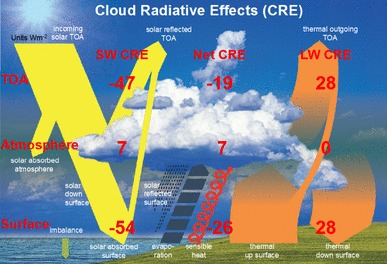
\includegraphics[scale = 7]{Chapter1_Intro/images/CRE_wild2019.jpg}
    \caption{Cloud radiative effect, CRE is the difference between the radiative components of the Clear sky radiative and the all sky. Modified version of as Figure 15 in \cite{Wild2019TheModels}. \textbf{pappa syns denne var grusomt vanskelig.}}
    \label{fig:cre}
\end{figure}

\begin{equation} \label{eq:cre_sw}
    CRE_{sw} = SW\uparrow_{clear-sky} - SW\uparrow_{all-sky}
\end{equation}

\begin{equation} \label{eq:cre_lw}
    CRE_{lw} = LW\uparrow_{clear-sky} - LW\uparrow_{all-sky}
\end{equation}

\begin{equation} \label{eq:stefan-boltzmann}
    F = \sigma \epsilon T ^4
\end{equation}

The physical properties causing the interaction with radiation is described below. Dense low level clouds reflect solar radiation. This is called the albedo effect. \textit{Albedo} being the ratio between reflected to incoming radiation. The higher number concentrations of droplets in a cloud the higher the total surface area of droplets. The more radiation gets reflected back into space. Clouds absorb longwave radiation and re-emits it. The absorbed radiation originates from the surface and is given by Stefan-Boltzmann forth-power law, see equation (\ref{eq:stefan-boltzmann}). The emissivity, $\epsilon$ depends on the (composition, compactness and surface roughness) of the medium. Water, snow and ice have different spectral emissivity (\cite{Huang2018ImprovedClimate}). Different parts of the globe are covered by different surfaces and \citeauthor{Huang2016AnSimulations} proved that assuming a constant surface emissivity effects the \acrshort{toa} polar energy budget. The greenhouse effect increases with the cloud altitude. Since high clouds have low temperatures and since the re-emitted radiation at a lower intensity than they absorbed. Researchers are still working on determine the emissivity of the different phases. Despite the uncertainties related to emissivity of the medium, the re-emitted radiation is of a lower intensity than what it absorb.

\section{Clouds in future climates} \label{sec:intro_cloud_future_climates}
\begin{figure}[h]
    \centering
    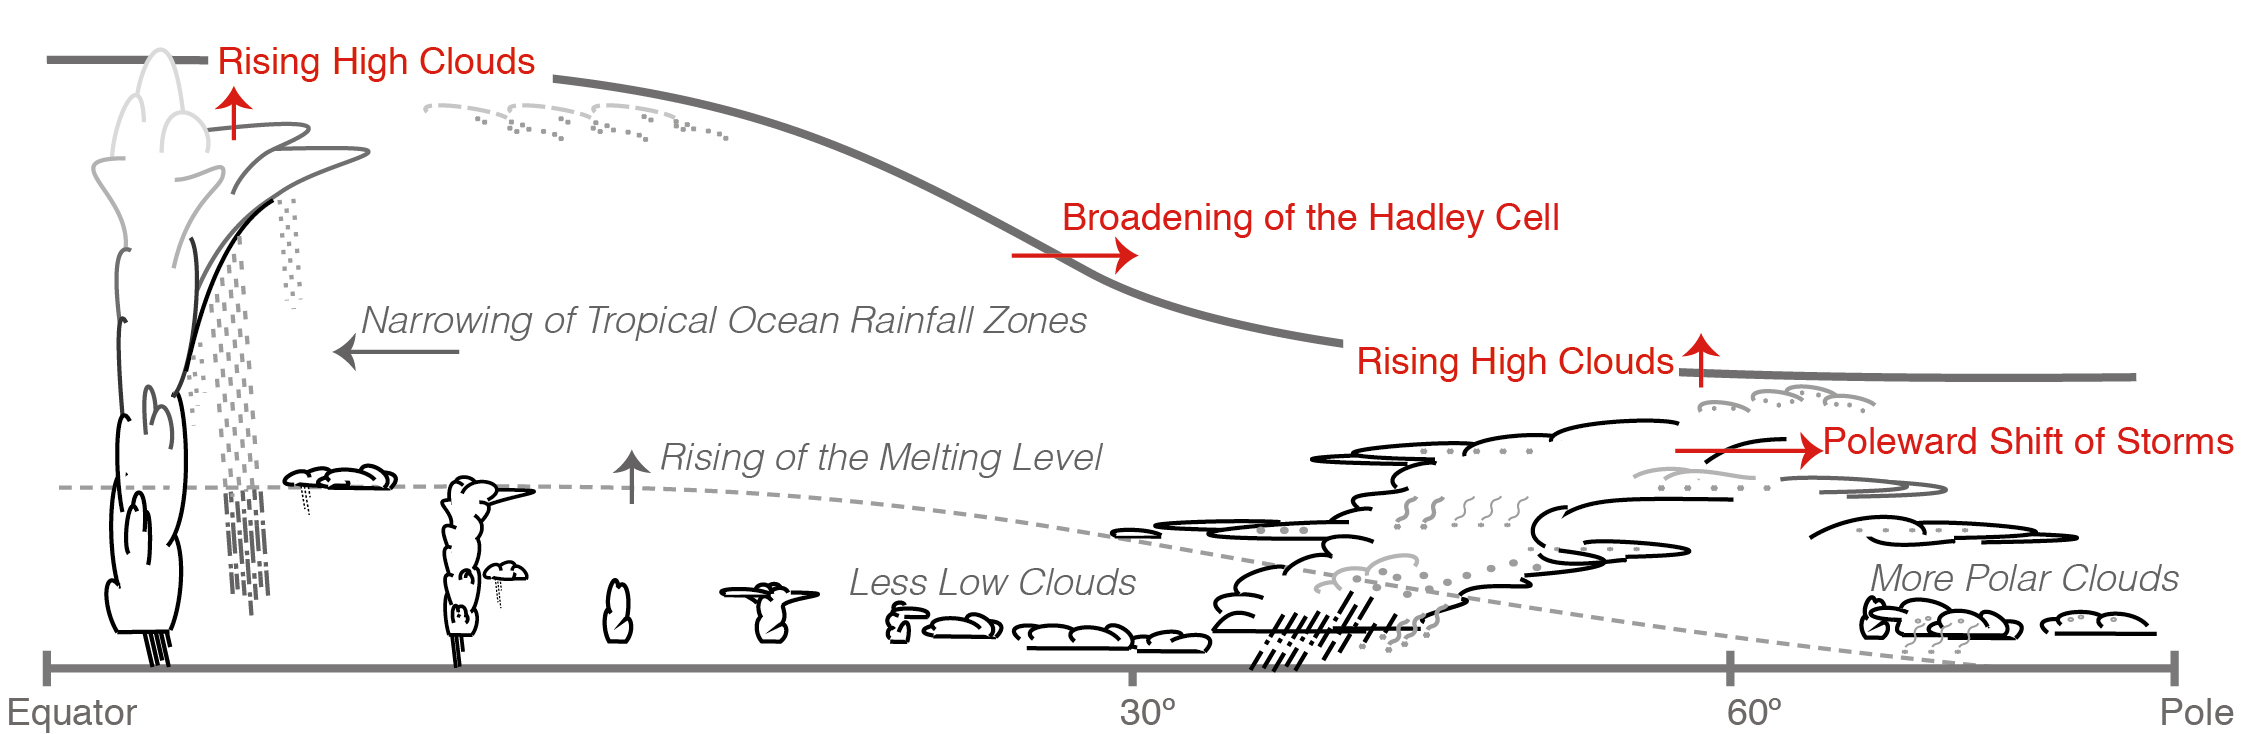
\includegraphics[scale = 0.8]{Chapter1_Intro/images/Fig7-11_ipcc.jpg}
    \caption{Cloud climatology in future climate. Developed based feedback's in climate models, the different adjustments have different uncertainty (\cite{IPCC_CH7_clouds}).}
    \label{fig:cloud_scheme}
\end{figure}

Excess of radiation gets trapped in the earth system, forcing the surface temperature to increase in order to close the radiative budget. The imbalance at the \acrfull{toa} is estimated by \cite{Wild2019TheModels} to be $0.6W m^{-2}$. 
% Wild et. al. 2019  \textbf{siter} finds an imbalance of This heat gets trapped in the earth system, forcing the surface temperature to increase in order to close the radiative budget. 
%The imbalance in the radiative budget at \acrfull{toa} is the radiative forcing. 
Climate drivers include both natural and anthropogenic forcings. \textit{Forcings} can be everything from natural variability in the solar energy output, volcanic eruptions and greenhouse gas emissions. The climate science community works toward a common goal to determine the climate sensitivity as a function of forcing. Different socio-economic pathways result different \acrshort{ecs}. The temperature increase induces climate changes. The \acrfull{ipcc} (\cite{IPCC_CH7_clouds}) suggest the following shift in cloud schemes (see figure \ref{fig:cloud_scheme}). Figure \ref{fig:cloud_scheme} shows a summary of the most likely cloud feedback's. First, a broadening of the Hadley cell causes a poleward shift of storms. This dries up the subtropics and moistens the higher latitudes. The clouds move further into the polar night, decreasing the albedo effect. The greenhouse effect of clouds still persist without sunlight leading to a net heating in the Arctic. Second, rising higher clouds causing a stronger greenhouse effect. Third, less low level clouds. This is assumed to be partly offset by a increase in the melting layer, leading to more opaque clouds. Rising of the meltlayer cause ice crystals to melt resulting in more opaque clouds. These opaque clouds have a higher albedo and reflect more sunlight. 
\section{Parametrization of clouds} \label{sec:param_clouds}
%\textit{In doing so, we do not include the effects of changes to the cloud microphysics explicitly.} Building a model based on meteorological variables provided by a reliable estimate from reanalysis datasets.
All global climate simulations are limited by computational power and the typical model grids are much too coarse to resolve all relevant processes governing clouds. Parameterization allows us to nevertheless simulate the effects of clouds on the climate, through simplified representations of cloud processes that are a function of resolved model variables. The development of both observational and modelling systems requires a understanding of the physical and biogeochemical processes that take place in the earth system (\cite{Simmons2016Observation2016-2025}). New ideas are implemented into models and tested. The simulated climate should be in accordance with observations and be able to recreate previous climate. 

The complex nature of clouds originates from lots of different processes occurring simultaneously on different scales. Incorporating all these interactions into a model framework has proven to be difficult (\cite{IPCC_CH9_climate_models}, \cite{IPCC_CH7_clouds} +++ ). \textbf{Finn multiple sources} 

% https://journals.ametsoc.org/doi/pdf/10.1175/2009JAS3072.1
% https://www.esrl.noaa.gov/psd/iasoa/vocabulary/Cloud%20Properties/Macrophysical
% Due to small scale of the processes involved, modelling the effects of clouds on the earth system requires parameterizations. 
% Due to the large uncertainty in \acrfull{ecs} related to clouds. 
%This area has received a lot of attention the last few years. A consequence of increasing the complexity of the models is the trailing increase in uncertainty. Popular approaches are saturation threshold, \acrfull{pdf} and \acrfull{crm}. 
%The data driven approach taken in this thesis does not net this case-specific adjustment. Doesn't need different approaches for different regimes, but relies on the satellites capabilities to detect them. Cirrus being the most difficult. When you one as seperate parameterizations for different cloud regimens, a consequence of this is that the cloud fraction might exceed 1.

\subsection{Relative humidity schemes}
The simplest form of cloud scheme is a binary. A model grid box is either cloudy or clear. Equation \eqref{eq:binary_param_clouds} describes a diagnostic relationship between cloud cover and relative humidity. Binary saturation threshold can be implemented as follows,
\begin{equation} \label{eq:binary_param_clouds}
    CFC\left(RH\right) = 
     \begin{cases}
       \text{0,} &\quad\text{if RH}\le100\\
       \text{1,} &\quad\text{else}
     \end{cases}
\end{equation}

\subsection{Statistical schemes}
Most climate models have a fractional cloud cover, which is driven by a saturation threshold. All the vapour in excess of this threshold, often $RH=100\%$, gets transformed into cloud liquid water. A representation of sub-grid scale variability is necessary to achieve fractional cloud cover. The most common variables either alone or in combination are relative humidity, temperature and vertical velocity (\cite{Golaz2002_part1}, ++ ).\textbf{cite more papers parametrizing this - draw inspiration from table?}  

Based on observations from airplane campaigns, researchers have attempted to draw statistical distributions of relevant variables. These \acrfull{pdf} are implemented into models. Virtually all existing \acrshort{pdf}s have been used to model either cloud cover or its dependent variables. % humidity, temperature and so on. 
%TS: Hva prøver du egentlig å si her over ("Virtually all...")? Jeg henger ikke helt med i resonnementet
A reproduction of the summary from \cite{Tompkins2009CloudParametrization}, describing distribution used in a selection of papers is given in Table \ref{tab:summary_PDF}.
\begin{table}[ht]
    \centering
    \setlength\tabcolsep{1.5pt} % default value: 6pt
    \setlength\extrarowheight{-7pt}
    \begin{tabular}{c|c|c}
        PDF shape &  Summary & Reference \\ \hline
        Double Delta & U, S & Ose (1993), Fowler et al. (1996) \\
        Uniform & U, S & LeTreut and Li (1991) \\
        Triangular & U, S & Smith (1990), Rotstayn (1997), Nishizawa (2000) \\
        Polynomial & U, S & Lohmann et al. (1999) \\
        Gaussian & U, S & Bougeault (1981), Ricard and Royer (1993) \\ 
        & &  Bechtolf et al. (1995) \\
        Beta & U, sk & Tomkins (2002) \\
        Log-normal & U, sk & Bony and Emanuel (2001) \\ 
        Exponential &  U, sk & Bougeault (1981), Ricard and Royer (1993) \\
        & &  Bechtolf et al. (1995) \\
        Double Gaussian/ Normal & B, sk & Lewellen and Yoh (1993), Golaz et al. (2002)
    \end{tabular}
    \caption{Reproduction of summary in \cite{Tompkins2009CloudParametrization}. Distributions used to parameterize cloud or its dependant variables. The key to decipher the summary column; U=Unimodal, B=Bimodal, S=Symmetric, sk = Skewed.}
    \label{tab:summary_PDF}
\end{table}
Researchers have not been successful in finding an adequate representation of cloud cover using these approaches (\cite{Tompkins2009CloudParametrization}). 

\cite{Golaz2002_part1} derived a joint \acrshort{pdf} of the sub-gridscale variability, serving as the base for parameterizing boundary layer clouds. This scheme is implemented in \acrfull{noresm} (\cite{SelandNORESM}) and \acrfull{cesm}, to recognised \acrshort{esm} (\cite{DanabasogluCESM}).
%TS: For NorESM kan du referere til Seland et al. (2002), og for CESM2 kan du referere til Danabasoglu et al. (2020)
The parameterization can be considered a higher-order turbulent closure problem. The first (mean), second (variance) and third order statistical moments, of the vertical velocity ($w$), the liquid water potential temperature ($\theta_l$), and the total water specific humidity ($q_t$) determines the family of \acrshort{pdf}s. It is designed to be flexible enough to (avoid the use of) circumvent the case specific adjustment. For more details see \cite{Golaz2002_part1} and \cite{Golaz2002_part2}.

%What is necessary to understand why clouds are Parameterisations. Cite that all climate models are wrong but some are useful.
\subsection{Cloud resolving models} \label{sec:params_climate_models}
Another method of cloud parameterization is using \acrfull{crm} that are integrated into global climate models. Contrary to what the name implies, this type of model still has problems with resolving the very smallest cloud processes, occurring on micrometer-scales. 

Running an \acrfull{les}-model, the increased resolution is able to resolve convective motions, but microphysical processes and turbulence effects still require parameterizations. \citeauthor{Baba2019SpectralModel} used this approach for parameterizing a spectral cumulus cloud. Obtaining the entrainment rate based on cloud properties from a \acrshort{crm} they built a parameterization valid for both shallow and deep convection. \textit{Entrainment rate} is the rate at which surrounding air penetrates the cloud. Preserving the physical properties, it is important that the method handles co-existing phenomena (\cite{Baba2019SpectralModel}). 

%Accelerating the speed of computations is always useful. 
\acrshort{dl} provides suitable methods for emulating %emulating what?, 
aimed to accelerate the speed of the heavy computations in \acrshort{crm}. Emulation in the context of computing refers to imitation of one model using another one. In this example the statistical models are used to mimic the behavior of the physically based \acrshort{crm}. The \acrshort{dl} model performance is restricted by the  \acrshort{crm}, performing at best as good as the \acrshort{crm} (\cite{Rasp2018DeepModels}).


\section{Data}
This section presents the data used in the compilation of the dataset, including background information about remote sensing of cloud properties and the method used to retrieve the data. 

\subsection{ERA5} \label{sec:era5}
ERA5 is the latest in the series of reanalyses produced by \acrfull{ecmwf}. Reanalysis is as close to observations as one can get while still obtaining data that is complete and coherent in both space and time. It is produced using a forecast model to assimilate observations. Data assimilation take observations as input and tries to make an accurate estimate of the state of the system that is as consistent as possible with the available observations at all times. This includes observations retrieved from satellites, ships, buoys, airplanes and ground-based stations. The analysis is produced in the operational forecast system, making it available within five days of real time. ERA5 is based on the Integrated Forecasting System, IFS cycle 4lr2. The data is available at a horizontal resolution of $0.25^o$ degree and hourly temporal resolution. It is an important product for the continuous monitoring of the Earth system 
(\cite{Hersbach2018OperationalStatus}).

Reanalyses data is often mistakenly referred to as observations. \citeauthor{Parker2016ReanalysesDifference} published an essay in \acrfull{bams} on this topic in \citeyear{Parker2016ReanalysesDifference}. Based on the following three points they conclude that observations and reanalyses are not too different. First, both involve inference, in other words, theory-based calculations. Second, reanalysis relies on forecast and observations do not. This is not a significant difference as long as the forecast is sufficiently accurate. Third, it is important to be aware that the uncertainty of the reanalyses is less well known than for observations. This makes it harder to judge the appropriate use of the reanalyses (\cite{Parker2016ReanalysesDifference}). 

\subsection{Remote sensing of cloud properties}
Satellites are the only instruments capable of providing continuous global measurements.
Measurements are collected by sensors, of which two types exist; passive and active imagers. The passive imaging sensors detect natural occurring levels of radiation, e.g. thermal radiation emitted by mediums. In contrast, active sensors  detect radiation returned from an emitted artificially fixed pulse of radiation (\cite{Stephens2018CloudsatSystem}). From \cite{Stockli2019CloudApplications}, \textit{the separation of the cloud from the cloud-free (reference signal) has been an everlasting problem in satellite-based cloud detection}.
\begin{figure*}
        \centering
        \begin{subfigure}[b]{0.475\textwidth}
            \centering
            \includegraphics[width=\textwidth]{Chapter2_Theory/images/sat_channels/meteosat-msg_wv062_overlay-ne_10m_coastline_overlay-ne_10m_admin_0_boundary_lines_land.png}
            \caption[Channel WV 6.2]%
            {{\small Channel WV 6.2}}    
            \label{fig:WV_6.2}
        \end{subfigure}
        \hfill
        \begin{subfigure}[b]{0.475\textwidth}  
            \centering 
            \includegraphics[width=\textwidth]{Chapter2_Theory/images/sat_channels/meteosat-msg_vis006_overlay-ne_10m_coastline_overlay-ne_10m_admin_0_boundary_lines_land.png}
            \caption[]%
            {{\small VIS 0.6}}    
            \label{fig:VIS_0.6}
        \end{subfigure}
        \vskip\baselineskip
        \begin{subfigure}[b]{0.475\textwidth}   
            \centering 
            \includegraphics[width=\textwidth]{Chapter2_Theory/images/sat_channels/meteosat-msg_ir108_overlay-ne_10m_coastline_overlay-ne_10m_admin_0_boundary_lines_land.png}
            \caption[something]%
            {{\small IR 10.8}}    
            \label{fig:IR_10.8}
        \end{subfigure}
        \quad
        \begin{subfigure}[b]{0.475\textwidth}   
            \centering 
            \includegraphics[width=\textwidth]{Chapter2_Theory/images/sat_channels/meteosat-msg_ir039_overlay-ne_10m_coastline_overlay-ne_10m_admin_0_boundary_lines_land.png}
            \caption{{\small IR 3.9}}    
            \label{fig:IR_3.9}
        \end{subfigure}
        \caption{{Spectral bands from SEVIRI. February 15th 2020 at noon. It shows the lowpressure system \textit{Elsa} positioned of the west coast of Iceland. Having a record breaking low of 915hPa (\cite{nrk_lavtrykk}). 
        The images are provided by  \cite{eumetcast_image_gallery}.}
    } 
    \label{fig:SEVIRI_channels}
\end{figure*}

% Info på bildene \textbf{Rectified (level 1.5) Meteosat SEVIRI image data. The data is transmitted as High Rate transmissions in 12 spectral channels. Level 1.5 image data corresponds to the geolocated and radiometrically pre-processed image data, ready for further processing, e.g. the extraction of meteorological products. Any spacecraft specific effects have been removed, and in particular, linearisation and equalisation of the image radiometry has been performed for all SEVIRI channels. The on-board blackbody data has been processed. Both radiometric and geometric quality control information is included. Images are made available with different timeliness according to their latency: quarter-hourly images if latency is more than 3 hours and hourly images if latency is less than 3 hours (for a total of 87 images per day). To enhance the perception for areas which are on the night side of the Earth a different mapping with increased contrast is applied for IR3.9 product. The greyscale mapping is based on the EBBT which allows to map the ranges 200 K to 300 K for the night and 250 K to 330 K for the day.}
% Lastet ned 16.02.2020.

\citepaper{Karlsson2015AdvancingData} list the five key properties for remote sensing of clouds using passive imagery, these will be explained drawing examples from Figure \ref{fig:SEVIRI_channels}, showing signals detected by \acrshort{msg} at the following four spectral bands: \acrshort{wv} 6.2, \acrshort{vis} 0.6, \acrshort{ir} 3.9 and \acrshort{ir} 10.8. High radiances are displayed in white and lower in darker colours. In general anything that appears bright has a higher reflection at the \acrshort{toa} than the surface.  Broken clouds typically give rise to scattered patterns or texture in images with otherwise homogeneous, ice-free ocean for instance. To summarise, the success of a screening is dependent on the illumination, the state of the surface and atmosphere (\cite{Karlsson2015AdvancingData}).  

Figure \ref{fig:WV_6.2} shows detected water vapour. Clouds appear bright in \acrfull{vis} and \acrfull{nir} channels. This is shown in Figure \ref{fig:VIS_0.6}. Exploiting the fact that clouds are not perfectly emitting black bodies. \textbf{Det mangler en overgang, dobbelsjekk om det er to sider av samme sak eller det er to channels.}
%TS: Enig i at det mangler noe her, jeg henger ikke med på resonnementet
Clouds are typically colder than the Earth's surface. Cirrus cloud are optically thin, but can be detected using split window channels (\acrshort{ir}10.8 and \acrshort{ir}12.0) differences (see Figure \ref{fig:IR_10.8}). 

Clouds consisting of liquid droplets reflect strongly in \acrfull{swir} and \acrfull{mwir}, as displayed in Figure \ref{fig:IR_3.9}. Here the Earth's surface, including snow and ice, appear dark. This allows for detection of low level clouds at night. 

Improved technologies allow for measuring new variables, one example of such advances is the use of active sensors. Active sensors provide a more refined image of vertical profiles and allows for the detection of cloud phase. Despite the limitations of passive sensors they provide useful historical information and in some cases higher spatial and temporal resolutions. One attempt to relate passive measurements with active measurement under the same meteorological conditions is the \textit{Afternoon constellation, A-Train} launched as a cooperation between several space agencies; \acrfull{nasa}, \acrlong{jaxa} and the french \acrfull{cnes}. This has provided a useful link between the different types of measurements (\cite{Stephens2018CloudsatSystem}). 

The number of spectral bands and footprint size (pixel resolution) determine the practical application of a particular satellite retrieval. Differences in swath width determine the frequency at a given position, determining the temporal resolution. The viewing angle affects the optical properties of the medium, and also its apparent position. \textit{Parallax} describes the apparent shift in position of a object, caused by moving the observer along an axis. This is a known issue in remote sensing. Positions of satellites are changed. Moving the observer (satellite) changes the apparent position of the measurement. 
High viewing angles may cause similar issues, in detection of high clouds. This factor is negligible when detecting low clouds (\cite{Joro2010ComparisonFinland}). 

Differences in sensitivity and retrieval algorithms contribute to a large spread in global mean cloud amount among different cloud products. This also explains the difficulties involved in using one cloud dataset to evaluate another one. In their assessment of global cloud datasets \citepaper{Stubenrauch2013AssessmentPanel} compared the global mean cloud cover of six datasets (ISCCP, PATMOS-x, MODIS-ST, MODIS-CE, AIR-LMD and TOVS Path-B). In this process they eliminating MISR and ATSR-GRAPE because of different observation times (see Table 3 in \citepaper{Stubenrauch2013AssessmentPanel} ) and two outlier datasets, HIRS-NOAA and POLDER. Their results show that the difference among the six datasets is of order 0.08. In contrast, local differences could be up to 0.4 (\cite{Stubenrauch2013AssessmentPanel}). 

%%%%%%%%%%%%%%% NOTAT I TILFELLE JEG TENKTE JEG BURDE INKLUDERT FLERE DETALJER OM FLERE DATASET.
%Cloud-Aerosol Lidar and Infrared Pathfinder Satellite Observations, CALISO is much used in other research because it gives a vertically resolved cloud (3D observations). This additional spatial information is provided on the expense of frequency and uncertainty. \textit{Reason why calipso is ruled out as a candidate. large uncertainty Stubenau} MODIS has low spatial resolution but high temporal resolution, one to two days. National Oceanic and Atmospheric Administration, NOAA \textbf{ something}. Most polar orbiting satellites have a resolution at best daily. \textbf{kilde (shubenau)} \textbf{Does the other one give ferdig produkter av skyfraksjoner og eller er mye lettere og regridde??} The number of channels (higher for other than METEOSAT). The more channels you have the more accurate cloud detection algorihms you can use. Most of the uncertainty in satellite retrivals are attributed to the presence of clouds.  

\subsection{METeosat Second Generation, MSG} \label{sec:meteosat}
The \acrfull{msg} was established as a corporation between \acrfull{esa} and \acrfull{eumetsat}. \acrshort{esa} was in charge of developing the prototype of MSG-1. \acrshort{eumetsat} is responsible for maintaining the user requirements, launch procedures, developing ground segments, ensuring overall system consistency and day to day operations. 

The primary function of \acrshort{msg} is to provide continuous observations of the Earth's full disk. Near-constant sampling frequency and a geostationary orbit allows for observing weather phenomena occurring on short timescales. Located at $0^o$ \arcshort{msg} provides a varying spatial resolution, unlike the polar orbiting satellites. The resolution gets coarser with increasing off-nadir viewing angle (\cite{Stubenrauch2013AssessmentPanel}). There are efforts invested in extending the MSG dataset with the \acrfull{mfg}, in order to make use of the time series all the way back to 1980. \textbf{kilde, launched 1977} This requires new cloud detection algorithms since they only have three common channels and only two of them are useful for detecting clouds (\cite{Stockli2019CloudApplications}). 

On board the \acrshort{msg} is the \acrfull{seviri} imaging radiometer. It has 12 spectral channels. The scan is done south to north, east to west. The wavelengths of the discrete channels are chosen based on heritage from other sensors. \arcshort{seviri} has one broadband visible channel, three solar channels (0.6, 0.8 and 1.6 $\mu m$) and 8 thermal infrared channels (3.9, 6.2, 7.3, 8.7, 9.7, 10.8, 12.0 and 13.4 $\mu m$) (\cite{Taravat2015MultilayerMasking}). This is of great advantage since much of the community already knows how to use the \acrshort{seviri} radiance observations. The channels have been chosen based on their ability to detect clouds, water vapour and ozone. More information about what the different channels detect is available in the paper \textit{An introduction to METeosat second generation (MSG)} published in \acrshort{bams} by \citepaper{Schmetz_meteosat_intro}.

Prior to the launch of the METeosat researchers discussed the temporal frequency suitable for observing weather phenomena. The METeosat first generation had a temporal resolution of 30min (\cite{Stockli2019CloudApplications}). For the second generation, 15min intervals were chosen to best cope with the short lifetime and rapid deformation of clouds. It was also suggested that a temporal frequency of 1 to 10min is necessary for tracking cumulus type clouds (\cite{Schmetz_meteosat_intro}). % 987 
This is in agreement with the Table 1.3 in \citeauthor{lohmann2016} (\citeyear{lohmann2016}, p. 19) stating the lifetimes of different types of clouds.

A \textit{ring} of geostationary satellites located at equator together provide global coverage (excluding polar regions). The altitude of the satellite determines its forward velocity. To achieve a geosynchronous orbit, a satellite needs to maintain a height of $\sim 36 000km$ (\cite{Bley2013ASEVIRI}).  

The first METeosat Second Generation (MSG-1) was launched 28 August 2002, and became operational 29 January 2004 when it was renamed METeosat-8. As a measure to reduce gaps, the \acrshort{msg} system provides a two-satellite system, one operational and one standby. The standby satellite scans when the operational satellite experiences technical failures. 
The operational satellite at nadir points at $0^o$ latitude. A full disk is $3712\times 3712$ pixels, and is sampled in cycles of 15min (\cite{Schmetz_meteosat_intro}).

\begin{figure}[h]
    \centering
    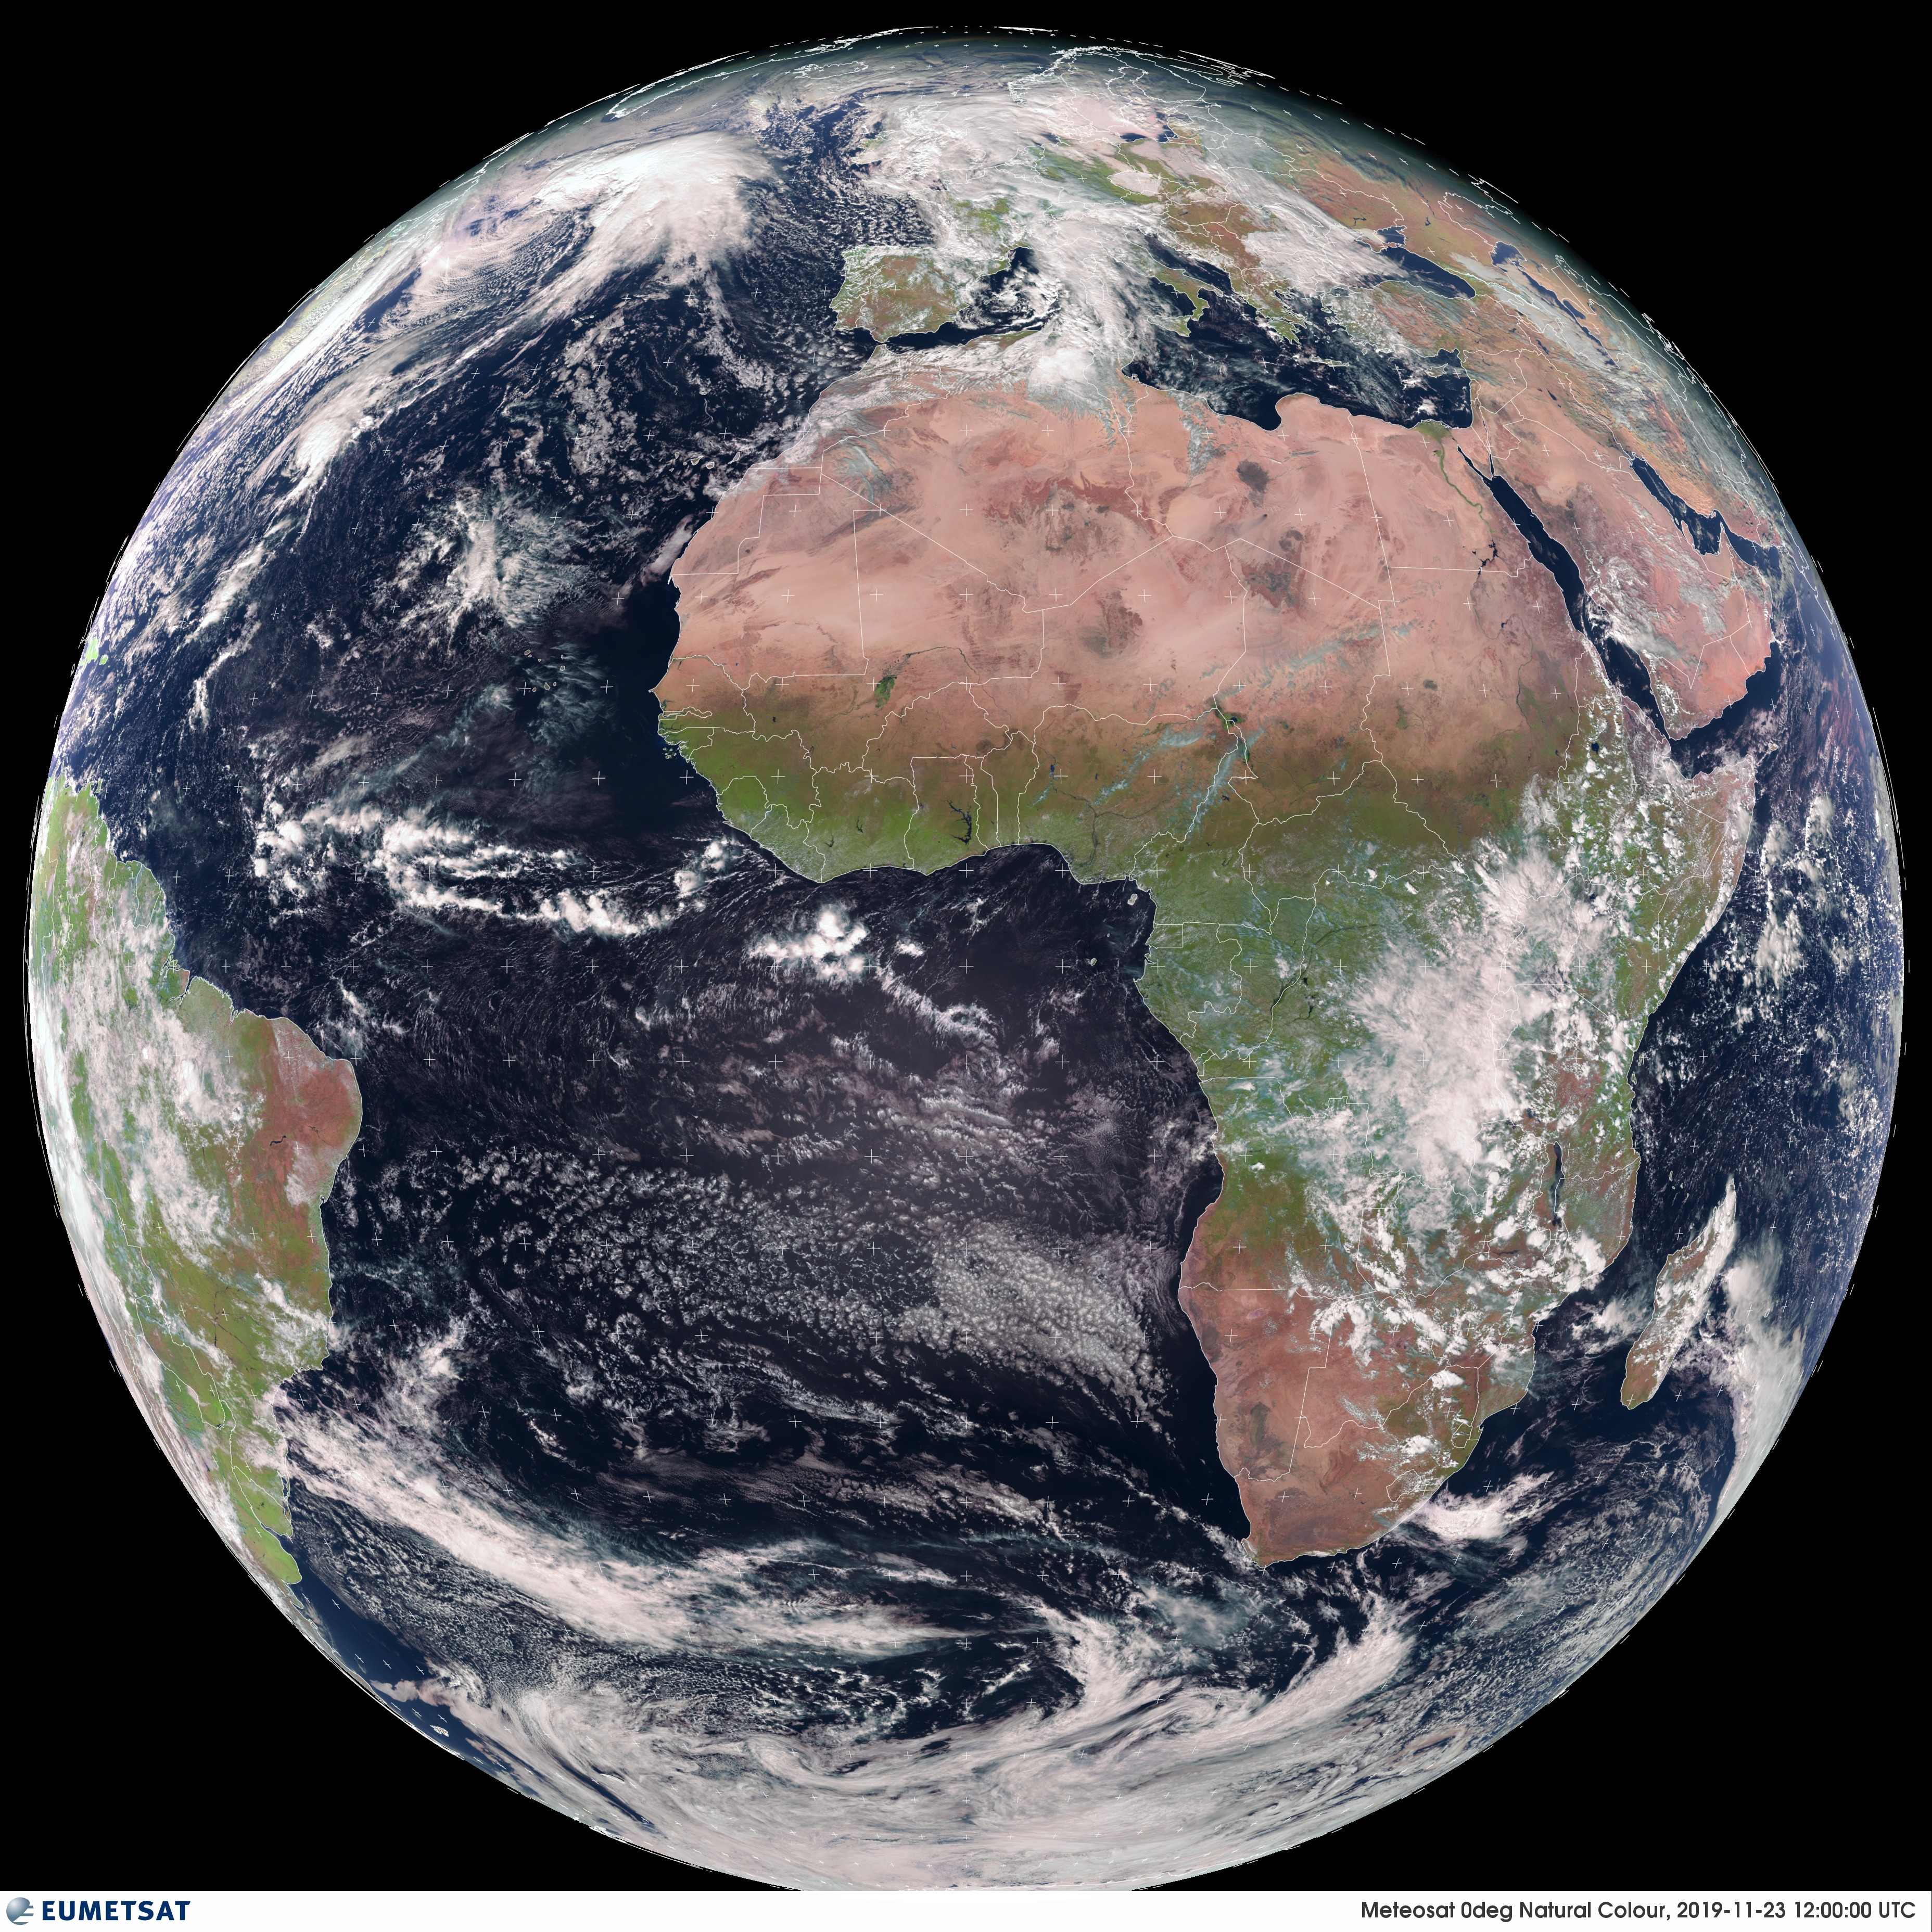
\includegraphics[scale=0.11]{Chapter2_Theory/images/MET10_RGBNatColourEnhncd_FullResolution_20191123120000.jpg}
    \caption{The view of Earth by \acrshort{seviri} on \acrshort{msg}, in naturally enhanced colours. This snapshot is dated noon 23rd of November 2019. By studying this image it becomes clear that clouds are influenced by circulation  (\cite{eumetcast_image_gallery}).}
    \label{fig:sat_view}
\end{figure}
The operational cloud detection algorithm is carried out pixel by pixel. Post processing involves re-classifying isolated pixels. There is a lot of effort invested in new detection algorithms including spatial structures. One of the methods that show potential here is deep learning (\cite{Dronner2018FastNetworks}, \cite{jeppesen_deep_cloud_masking}).

\subsection{EUMETSAT Cloud Mask} \label{sec:EUMETSAT_cloud_mask}
The \acrshort{eumetsat} cloud mask, CLM consist of four classes, described in Table \ref{tab:classes_clm}.
\begin{table}[]
    \centering
    \setlength\extrarowheight{-7pt}
    \begin{tabular}{c|c}
        Class & Description \\ \hline
        0 & Clear sky over ocean \\
        1 & Clear sky over land \\
        2 & Cloudy \\
        3 & No data/ outer space        
    \end{tabular}
    \caption{Description of classes in EUMETSAT Cloud Mask product.}
    \label{tab:classes_clm}
\end{table}
\begin{table}[]
    \centering
    \setlength\extrarowheight{-7pt}
    \begin{tabular}{c|c}
        Spectral band & Central wavelength $\left( \mu m  \right)$ \\ \hline
        VIS 0.6 & 0.635 \\
        VIS 0.8 & 0.81 \\
        NIR 1.6 & 1.64 \\
        IR 3.9 & 3.92 \\
        WV 6.2 & 6.25 \\
        WV 7.3 & 7.35 \\ 
        IR 8.7 & 8.7 \\
        IR 9.7 & 9.66 \\
        IR 10.8 & 10.8 \\
        IR 12.0 & 12 \\
        IR 13.4 & 13.4 \\
        HRV & 0.75
    \end{tabular}
    \caption{Summary of spectral bands, central wavelength and their respective retrieval abilities (\cite{Schmetz_meteosat_intro}).}
    \label{tab:msg_spectral_bands}
\end{table}
These classes are derived from almost all channels except the broadband HRV and isolated pixels are reclassified \textbf{cite article 10 in Tavarat, 2015}. The cloud mask is distributed in \acrfull{grib},  without coordinates and \acrfull{netcdf}, processed with coordinates and reshaped into the standard rotation, as displayed i Figure \ref{fig:sat_view} The data is available via Earth Observation Portal on EUMETSATS web pages. 

\clearpage
\subsection{WHY I CHOSE COMBINATION OF REANALYSIS AND msg - FEIL PLASS?}
Using reanalysis data for the envionmental variable is a clear choice, there is no other products providing gridded data, coherent in time and space. 

Satelite data is the only platform (?) providing (almost) simultaneous global measurments, necessary for this task. 
Having demonstrated its usefullness for task of \textbf{Les i \cite{Stockli2019CloudApplications}}.
Secondly, the usefulness of rapid scans was given hight priority when making the choices for the databasis of \acrshort{ecc}. This has been demonstrated for nowcasting and other application \textbf{add citations from \cite{Stockli2019CloudApplications}}.
%TS: Vel, det hadde i hvert fall vært bra å forklare hvorfor valget falt på dette datasettet